% !TEX root = Dokumentation.tex
\section{Projektführung}
Die nachfolgenden Abschnitte dienen der Projektführung und sollen das Projektmanagement unterstützen. Dabei werden der zeitliche Rahmenplan erläutert und die Risiken im Zusammenhang mit dem Projekt beleuchtet.
\subsection{Rahmenplan}
Um einen Überblick über den geplanten Projektverlauf zu bekommen, ist nachfolgend
ein Rahmenplan definiert.
\begin{figure}[H]%Position festigen
\centering
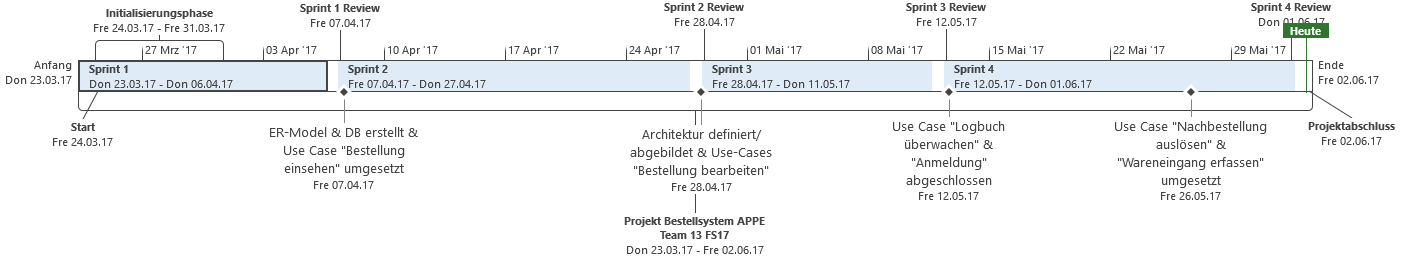
\includegraphics[width=1.0\textwidth]{Images/GroberTerminplan.png}
\label{fig:title}
\end{figure}
Das Projekt wird vom 23.03.2017 bis am 02.06.2017 durchgeführt. Zur regelmässigen Kontrolle \↨& Planung wird die Projektdauer in vier Entwicklungssprints unterteilt. Auf dem Weg zur finalen Version werden ebenfalls vier Meilensteine wie folgt gesetzt:
\begin{enumerate}
\item Meilenstein 1 \textit{ER-Modell \& DB erstellt \& Use Case 'Bestellung einsehen' umgesetzt}\\
Neben den Initialisierungsaufgaben wie Erstellung PMP \& SysSpec und initiale Anforderungsaufnahme liegt die DB anhand des vorgängig erstellten ER-Modell vor. Weiter ist der erste Use Case 'Bestellung einsehen' umgesetzt
\item Meilenstein 2 \textit{Architektur definiert \& Use Case 'Bestellung bearbeiten' umgesetzt}\\
Neben der Layer- \& Tierarchitektur, Komponentenschnitt ist der Use Case 'Bestellung bearbeiten' vollständig umgesetzt. 
\item Meilenstein 3 \textit{Use Case 'Nachbestellung' \& 'Anmeldung' umgesetzt} \\
Alle Use Cases bis auf 'Logbuch überwachen' sind umgesetzt. Erste Integrations- \& Systemtests sind ausgeführt.
\item Meilenstein 4 \textit{Use Case 'Logbuch überwachen' \& Dokumentation abgeschlossen}\\
Neben dem letzten Use Case 'Logbuch überwachen' werden alle Integrations- \& Systemtests durchgeführt. Abschliessend liegen die SysSpec und der PMP vor.
\end{enumerate}

\subsubsection{Projektkontrolle}
In der Projektkontrolle sollen Abweichungen zwischen SOLL- und IST-Zustand aufgedeckt werden. Der Zustand bezieht sich auf den Projektfortschritt. In jedem Sprint werden Arbeitspakete definiert und mit einem bestimmten Aufwand (in Stunden) versehen
\subsubsection{Risikomanagement}

\subsubsection{Projektabschluss}